\documentclass{jarticle}
\usepackage[dvipdfmx]{graphicx}
\usepackage{here}
\usepackage{listings,jlisting}


\lstset{
  basicstyle={\ttfamily},
  identifierstyle={\small},
  commentstyle={\smallitshape},
  keywordstyle={\small\bfseries},
  ndkeywordstyle={\small},
  stringstyle={\small\ttfamily},
  frame={tb},
  breaklines=true,
  columns=[l]{fullflexible},
  numbers=left,
  xrightmargin=0zw,
  xleftmargin=3zw,
  numberstyle={\scriptsize},
  stepnumber=1,
  numbersep=1zw,
  lineskip=-0.5ex
}

\title{{システム実験}\\実験8回レポート}
\author{6119019056 山口力也}
\date{2019/06/14日提出}

\begin{document}
\maketitle

\section{レポート4.1.1}
課題4.1.1で作成したArduinoスケッチとProcessingスケッチを報告せよ.また本課題を行った結果(グラフのスナップショットを含む)を報告せよ.

以下ソースコード\ref{code:kadai4-1-1-a}にArduinoのスケッチを,ソースコード\ref{code:kadai4-1-1-p}にProcessingのスケッチを示す.

\begin{lstlisting}[caption = 課題4.1.1(Arduino),label=code:kadai4-1-1-a][H]
int sensorValue0, sensorValue1;
unsigned long int timeNow,timePrev;
int inByte; // Processing から の送信要求を 受け 取る 変数
void setup(){
  Serial.begin(9600);
}
void loop(){
  timeNow = millis();
  sensorValue0 = analogRead(0);
  if (Serial.available() > 0) {
    if ( timeNow - timePrev >= 50 ) {// 送信要求を 受け 取っ た ( 受信バッ フ ァ に データ あり )
      inByte = Serial.read(); // 受信済みの信号を 読み込む ( 受信バッ フ ァ が空に な る )
      Serial.write(252); //はじめの位置確認
      Serial.write(sensorValue0 / 0x20);
      Serial.write(sensorValue0 % 0x20);

      Serial.write(timeNow >> 28); //1byte目
      Serial.write(timeNow >> 21); //2byte目
      Serial.write(timeNow >> 14); //3byte目
      Serial.write(timeNow >> 7);  //4byte目
      Serial.write(timeNow && 127); //5byte目
      timePrev = timeNow;
    }
  }
  
}
\end{lstlisting}

\begin{lstlisting}[caption = 課題4.1.1(Processing),label=code:kadai4-1-1-p][H]
import processing.serial.*;
Serial port;
int val;
int x,y;
int time,time_min,time_max;
int period;
int byte1,byte2,byte3,byte4,byte5;
void setup(){
  size(1200, 500); //サイズウィンドウ
  port = new Serial(this, "/dev/ttyUSB0", 9600);
  period = 20000;
  time_min = 0;
  time_max = period;
  x = 0; y= 0;
  background(255);
  frameRate(60);
 }
void draw(){
  if ( time > time_max ) {
    time_min += period;
    time_max += period;
    background(255);
  }
  x = (int)map(time,time_min,time_max,0,width); //線形変換
  y = (int)map(val,0,1023,height,0); //線形変換
  stroke(255,0,0); //文字色指定
  ellipse(x,y,5,5); //円を描画
}
void serialEvent(Serial p){
  if (p.available() >= 8) {
    if (p.read() == 252) {
      val = p.read() * 0x20 + p.read(); //値読み込み
      byte1 = p.read(); //時間の1byte目
      byte2 = p.read(); //時間の2byte目
      byte3 = p.read(); //時間の3byte目
      byte4 = p.read(); //時間の4byte目
      byte5 = p.read(); //時間の5byte目
      time = (byte1 << 28 )+ (byte2 << 21) + (byte3 << 14 ) + (byte4 << 7 ) + byte5 ; //5バイト
      println(val);
      
      port.write(0xff); // 次のデータ 送信要求 ( 任意の 1 バイ ト ) を 送信
    }
  }
}
void mousePressed(){ //マウスボタンが押されたら割り込み
  port.write(0xff);
}
\end{lstlisting}

また,以下図\ref{fig:kadai4-1-1}にグラフのスナップショットを示す.

\begin{figure}[H]
\begin{center}
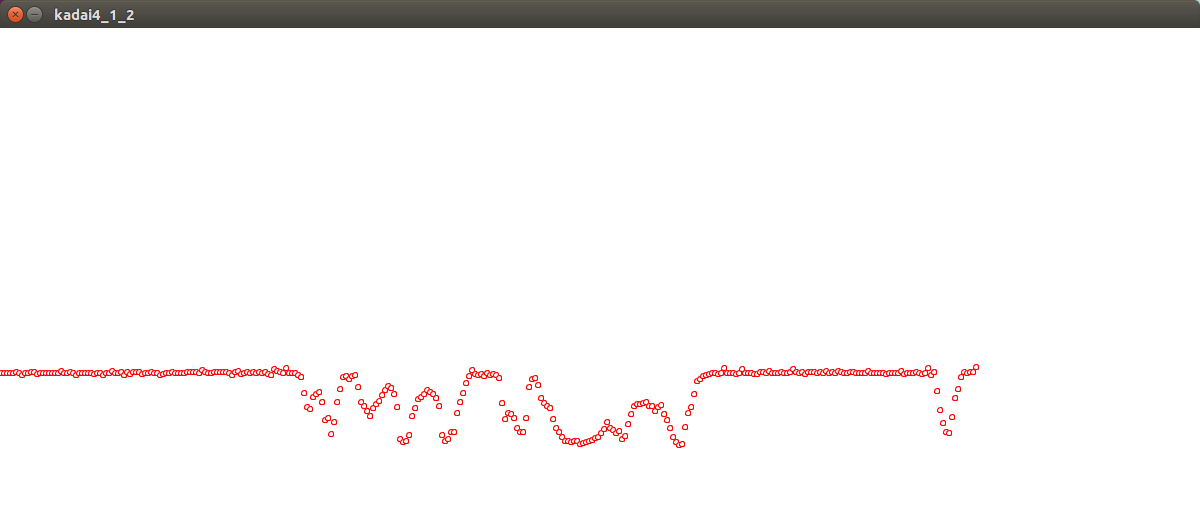
\includegraphics[width=10.0cm]{images/kadai4-1-1.png}
\caption{課題4-1-1の出力画像}
\label{fig:kadai4-1-1}
\end{center}
\end{figure}


\section{レポート4.1.2}
課題4.1.2で作成したArduinoスケッチとProcessingスケッチを報告せよ.また本課題を行った結果(グラフのスナップショットを含む)を報告せよ.

以下ソースコード\ref{code:kadai4-1-2-a}にArduinoのスケッチを,ソースコード\ref{code:kadai4-1-2-p}にProcessingのスケッチを示す.

\begin{lstlisting}[caption = 課題4.1.2(Arduino),label=code:kadai4-1-2-a][H]
int sensorValue0, sensorValue1;
unsigned long int timeNow,timePrev;
int inByte; // Processingからの送信要求を受け取る変数
const int LED = 13;
int byte1,byte2,byte3,byte4;
void setup(){
  Serial.begin(9600);
}
void loop(){
  timeNow = millis();
  sensorValue0 = analogRead(0);
  if (Serial.available() > 0) {
    if ( timeNow - timePrev >= 50 ) {// 送信要求を受け取った
      inByte = Serial.read(); // 受信済みの信号を読み込む 
      Serial.write(252); //はじめの位置確認
      Serial.write(sensorValue0 / 0x20);
      Serial.write(sensorValue0 % 0x20);
      byte1 = timeNow >> 28;
      byte2 = timeNow >> 21;
      byte3 = timeNow >> 14;
      byte4 = timeNow >> 7;
      Serial.write(byte1 & 0x7F); //1byte目
      Serial.write(byte2 & 0x7F); //2byte目
      Serial.write(byte3 & 0x7F); //3byte目
      Serial.write(byte4 & 0x7F);  //4byte目
      Serial.write(timeNow & 0x7F); //5byte目
      timePrev = timeNow;
      digitalWrite(LED,HIGH);
    }
  }
  if ( Serial.available() == 0) {
    digitalWrite(LED,LOW);
    if ( timeNow - timePrev >= 1000 ){  
      inByte = Serial.read(); // 受信済みの信号を読み込む
      Serial.write(252); //はじめの位置確認
      Serial.write(sensorValue0 / 0x20);
      Serial.write(sensorValue0 % 0x20);
      byte1 = timeNow >> 28;
      byte2 = timeNow >> 21;
      byte3 = timeNow >> 14;
      byte4 = timeNow >> 7;
      Serial.write(byte1 & 0x7F); //1byte目
      Serial.write(byte2 & 0x7F); //2byte目
      Serial.write(byte3 & 0x7F); //3byte目
      Serial.write(byte4 & 0x7F);  //4byte目
      Serial.write(timeNow & 0x7F); //5byte目
      timePrev = timeNow;
      digitalWrite(LED,HIGH);
    }
  }
}
\end{lstlisting}

\begin{lstlisting}[caption = 課題4.1.2(Processing),label=code:kadai4-1-2-p][H]
import processing.serial.*;
Serial port;
int val;
int x,y;
int time,time_min,time_max;
int period;
int byte1,byte2,byte3,byte4,byte5;
void setup(){
  size(1200, 500);
  port = new Serial(this, "/dev/ttyUSB0", 9600);
  period = 20000;
  time_min = 0;
  time_max = period;
  x = 0; y= 0;
  background(255);
  frameRate(60);
 }
void draw(){
  if ( time > time_max ) { //時間更新
    time_min += period;
    time_max += period;
    background(255);
  }
  x = (int)map(time,time_min,time_max,0,width);
  y = (int)map(val,0,1023,height,0);
  stroke(255,0,0);
  ellipse(x,y,5,5);
}
void serialEvent(Serial p){
  if (p.available() >= 8) {
    if (p.read() == 252) {
      val = p.read() * 0x20 + p.read();
      byte1 = p.read(); //時間の1byte目
      byte2 = p.read(); //時間の2byte目
      byte3 = p.read(); //時間の3byte目
      byte4 = p.read(); //時間の4byte目
      byte5 = p.read(); //時間の5byte目
      time = (byte1 << 28 )+ (byte2 << 21) + (byte3 << 14 ) + (byte4 << 7 ) + byte5 ; //5バイト
      println(val);
      println("time=",time);
      port.write(0xff); // 次のデータ送信要求
    }
  }
}
void mousePressed(){ //マウスボタンが押されたら割り込み
  port.write(0xff);
}
\end{lstlisting}

また,以下図\ref{fig:kadai4-1-2}にグラフのスナップショットを示す.

\begin{figure}[H]
\begin{center}
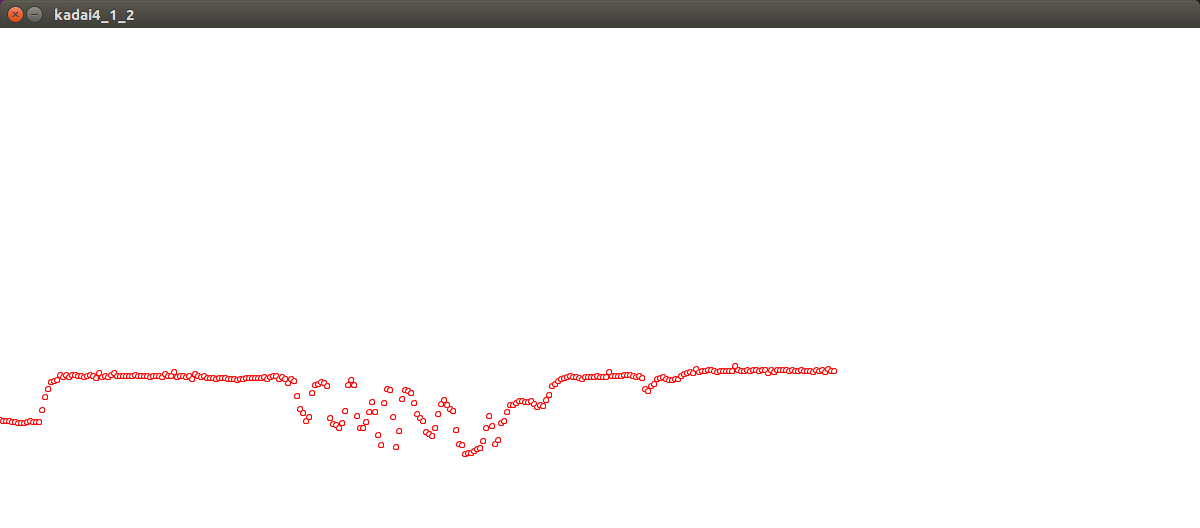
\includegraphics[width=10.0cm]{images/kadai4-1-2.png}
\caption{課題4-1-2の出力画像}
\label{fig:kadai4-1-2}
\end{center}
\end{figure}

\section{レポート4.1.3}
課題4.1.3で作成したグラフのスナップショットを報告せよ.ただし,Arduinoを移動させてデータを取得し,一時的にデータ通信が途切れている状況を含むようにすること.
以下図\ref{fig:kadai4-1-2}に出力したcsvファイルから作成したグラフを示す.

\begin{figure}[H]
\begin{center}
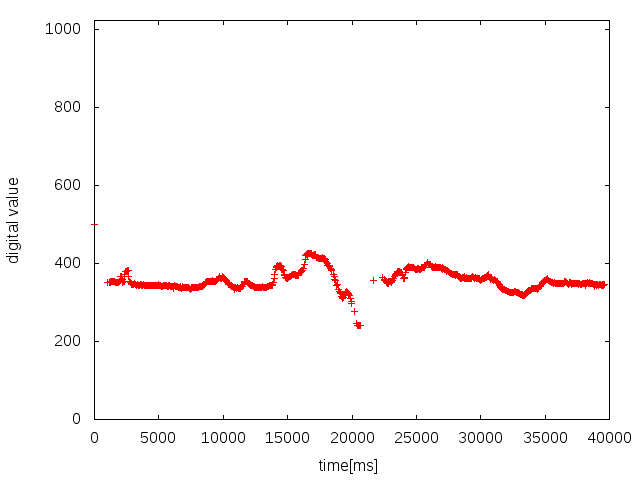
\includegraphics[width=10.0cm]{images/kadai4-1-3-graph.png}
\caption{課題4-1-3のグラフ画像}
\label{fig:kadai4-1-2}
\end{center}
\end{figure}

\section{レポート4.1.4}
課題4.1.4で作成したArduinoスケッチとProcessingスケッチを報告せよ.また本課題を行った結果(グラフのスナップショットを含む)を報告せよ.

以下ソースコード\ref{code:kadai4-1-4-a}にArduinoのスケッチを,ソースコード\ref{code:kadai4-1-4-p}にProcessingのスケッチを示す.

\begin{lstlisting}[caption = 課題4.1.4(Arduino),label=code:kadai4-1-4-a][H]
int Luxsensor, Tempsensor;
long int Luxsum,Tempsum,count;
float Luxaverage,Tempaverage;
unsigned int intLuxaverage,intTempaverage;
unsigned long int timeNow,timePrev;
int byte1,byte2,byte3,byte4;
int inByte; // Processing から の送信要求を 受け 取る 変数
void setup(){
  Serial.begin(9600);
  timePrev = millis();
  Luxsum = 0;
  Tempsum = 0;
  count = 0;
}
void loop(){
    timeNow = millis();
    Luxsensor = analogRead(0); a0ポートの値を読み込み
    Tempsensor = analogRead(1); a1ポートの値読み込み
    if ( (timeNow - timePrev) <= 50 ) { //50ms経つまで
        Luxsum += Luxsensor; //足し込む
        Tempsum += Tempsensor; //足し込む
        count ++;
    }
    else {
    Luxaverage = (float)Luxsum / (float)count *100; //平均値をとる
    Tempaverage = (float)Tempsum / (float)count *100; //平均値を取る
    intLuxaverage = (int)(Luxaverage); //int型にキャスト
    intTempaverage = (int)(Tempaverage); //int型にキャスト
    inByte = Serial.read();
    Serial.write(0x20); //はじめの位置確認
    Serial.write(intLuxaverage / 0x50);
    Serial.write(intLuxaverage % 0x50);
    Serial.write(intTempaverage / 0x50);
    Serial.write(intTempaverage % 0x50);
    /*
    Serial.println(Tempaverage);
    Serial.println(Luxaverage);
    Serial.println(intTempaverage);
    Serial.println(intLuxaverage);
    */
    byte1 = timeNow >> 28;
    byte2 = timeNow >> 21;
    byte3 = timeNow >> 14;
    byte4 = timeNow >> 7;
    Serial.write(byte1 & 0x7F); //1byte目
    Serial.write(byte2 & 0x7F); //2byte目
    Serial.write(byte3 & 0x7F); //3byte目
    Serial.write(byte4 & 0x7F);  //4byte目
    Serial.write(timeNow & 0x7F); //5byte目
    timePrev = timeNow;
    count = 0;
    Luxsum = 0;
    Tempsum = 0; 
    }
}
\end{lstlisting}

\begin{lstlisting}[caption = 課題4.1.4(Processing),label=code:kadai4-1-4-p][H]
import processing.serial.*;
Serial port;
PrintWriter output; //PrintWriterクラスのオブジェクトを宣言
float val_lux,val_temp;
int sum_lux,sum_temp;
int x,y1,y2;
int time,time_min,time_max;
int period;
int byte1,byte2,byte3,byte4,byte5;
void setup(){
  size(1200, 500);
  port = new Serial(this, "/dev/ttyUSB0", 9600);
  period = 20000;
  time_min = 0;
  time_max = period;
  x = 0; y1= 0; y2 = 0;
  background(255);
  frameRate(60);
  output = createWriter("kadai4-1-4.csv");
 }
void draw(){
  if ( time > time_max ) {
    time_min += period;
    time_max += period;
    background(255);
  }
  x = (int)map(time,time_min,time_max,0,width);
  y1 = (int)map(val_lux,0,1023,height,0);
  y2 = (int)map(val_temp,170,200,height,0);
  stroke(255,0,0);
  ellipse(x,y1,5,5);
  stroke(0,0,255);
  ellipse(x,y2,5,5);
}
void serialEvent(Serial p){
  if (p.available() >= 10) {
    if (p.read() == 0x20) {
      sum_lux = p.read() * 0x50 + p.read();
      sum_temp = p.read() * 0x50 + p.read();
      val_lux = (float)sum_lux / 100;
      val_temp = (float)sum_temp / 100;
      byte1 = p.read();
      byte2 = p.read();
      byte3 = p.read();
      byte4 = p.read();
      byte5 = p.read();
      time = (byte1 << 28 )+ (byte2 << 21) + (byte3 << 14 ) + (byte4 << 7 ) + byte5; //5バイト
      println("y1=",y1);
      println("val_lux=",val_lux);
      println("y2=",y2);
      println("val_temp=",val_temp);
      println("time=",time);
      port.write(0xff); // 次のデータ 送信要求 ( 任意の 1 バイ ト ) を 送信
    }
  }
}
/*
void mousePressed(){ //マウスボタンが押されたら割り込み
  port.write(0xff);
}
*
\end{lstlisting}

また,以下図\ref{fig:kadai4-1-4}にグラフのスナップショットを示す.

\begin{figure}[H]
\begin{center}
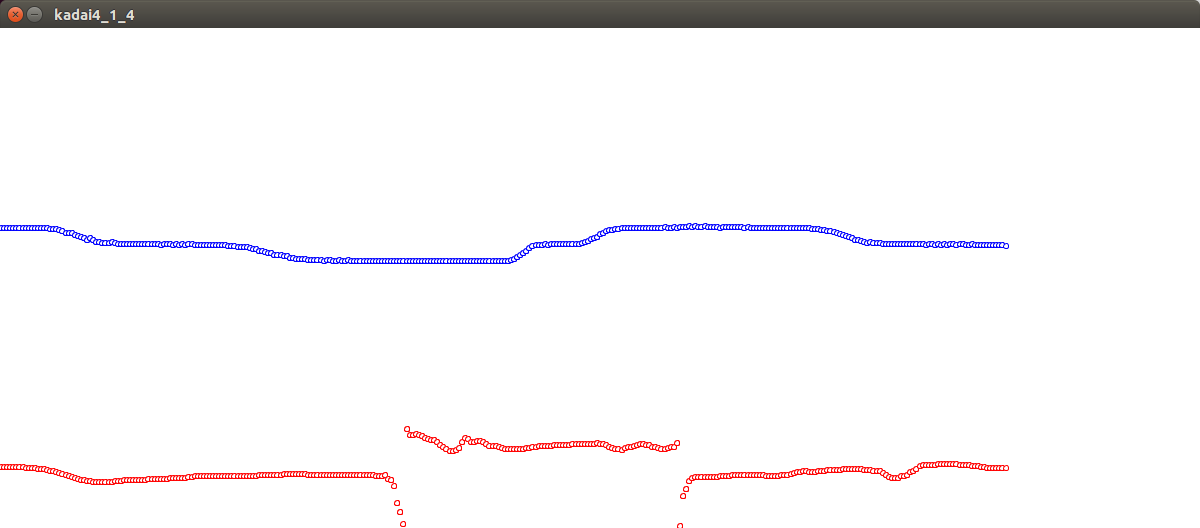
\includegraphics[width=10.0cm]{images/kadai4-1-4.png}
\caption{課題4-1-4の出力画像}
\label{fig:kadai4-1-4}
\end{center}
\end{figure}


\end{document}
